\subsection{Overzicht van wiskundige notaties}

\subsubsection{Vergelijkingen en ongelijkheden}

\begin{center}
	\begin{tabular}{lll}
	Notaties & Uitleg & Voorbeeld \\
	\hline
	$=$ & is gelijk aan & $3=1+2$ \\
	$\ne$ & is niet gelijk aan of verschillend van & $3\ne1+1$ \\
	$<$ & is strikt kleiner dan & $2<3$ \\
	$>$ & is strikt groter dan & $3>2$ \\
	$\le$ & is kleiner dan of gelijk aan & $3\le 4$ maar ook $4\le 4$ \\
	$\ge$ & is groter dan of gelijk aan & $4\ge 3$ maar ook $4\ge 4$ \\
	$\approx$ & is ongeveer gelijk aan & $\pi \approx 3$ \\
	$\sim$ & is recht evenredig met; is proportioneel met & straal van een cirkel $\sim$ \\
	& (als de grootheid links stijgt, & omtrek van een cirkel \\
	& stijgt de grootheid rechts even sterk) & \\
	$\iff$ & als en slechts als; is equivalent met & $x-1=0 \iff x=1$ \\
	\end{tabular}
\end{center}

\subsubsection{Bewerkingen en rekenen}

\begin{center}
	\begin{tabular}{lll}
		Notaties & Uitleg & Voorbeeld \\
		\hline
		$+$ & positief, plus of som & $+5, \ 1+3=4$ \\
		$-$ & negatief, min of aftrekking & $-5,\ 3-1=2$ \\
		$\cdot$ & maal of het product van & $2\cdot3=6$ \\
		$/$ (soms ook $:$) & teller gedeeld door noemer = quoti\"ent & $6/2=3$ \\
		$\pm$ & plusminus, boven en ondergrens & $10 \pm 1$ betekent  \\
		& (wordt gebruikt bij meetfouten) & $10+1$ en $10-1$ \\
		$| \ |$ & de absolute waarde van & $|-3|=|3|=3$ \\
		$\sqrt{\ }$ & de vierkantswortel van & $\sqrt{9}=3$ \\
		$!$ & faculteit & $3!=3\cdot2\cdot1=6$
	\end{tabular}
\end{center}

\subsubsection{Verzamelingen}

\begin{center}
	\begin{tabular}{lll}
		Notaties & Uitleg & Voorbeeld \\
		\hline
		$\in$ & is een element van & $3 \in \mathbb{N}$ \\
		$\notin$ & is geen element van & $-1 \notin \mathbb{N}$ \\
		$(\ ,\ )$ & een koppel; $xy$-co\"ordinaten & $(0,1)$ \\
		$[\ ,\ ]$ & gesloten interval & $x \in [3,5]\iff x\ge 3 \text{ en } x \le 5$\\
		$]\ ,\ [$ & open interval & $x \in ]3,5[\iff x> 3 \text{ en } x < 5$\\
		$[\ ,\ [$ & half open interval langs rechts & $x \in [3,5[\iff x\ge 3 \text{ en } x < 5$\\
		$]\ ,\ ]$ & half open interval langs links & $x \in ]3,5]\iff x> 3 \text{ en } x \le 5$\\
		$\subset$ & is een deelverzameling van & $\{0,2\} \subset \{0,1,2,3\}$ \\
		& & $\mathbb{N} \subset \mathbb{Z} \subset \mathbb{Q} \subset \mathbb{R} \subset \mathbb{C}$ \\
		$\cap$ & doorsnede & $\{0,1,2\} \cap \{2,3\} = \{2\}$\\
		& & $\{0,2,4,\ldots\}\cap\{1,3,5,\ldots\}=\{\}=\emptyset$\\
		$\cup$ & vereniging of unie & $\{0,1,2\}\cup \{2,3\} = \{0,1,2,3\}$\\
		$\setminus$ & verschil (van verzamelingen) & $\{0,1,2,3\} \setminus \{0\} = \{1,2,3\}$ \\
		$\{\}=\emptyset$ & de lege verzameling & Geen getal voldoet dus $x \in \emptyset$ \\
		$|$ & waarvoor geldt & De natuurlijke getallen die even zijn: \\
		& & $\{n \in \mathbb{N} | n \text{ is even}\}$
	\end{tabular}
\end{center}

\subsubsection{Bekende getallen en verzamelingen}

\begin{center}
	\begin{tabular}{lll}
		Notaties & Uitleg & Voorbeeld \\
		\hline
		$i$ & de imaginaire eenheid & $i^2=-1$ \\
		$\pi$ & het getal pi & $\pi=3,14159\ldots$ \\
		$e$ & het getal van Euler & $e=2,71828\ldots$\\
		& (wordt gebruikt bij exponenti\"ele & \\
		&  en logaritmische functies) & \\
		$\mathbb{N}$ & verzameling der natuurlijke getallen & $\mathbb{N}=\{0,1,2,3,\ldots\}$ \\
		$\mathbb{Z}$ & verzameling der gehele getallen & $\mathbb{Z}$=\{\ldots-3,-2,-1,0,1,2,3\ldots\}\\
		$\mathbb{Q}$ & verzameling der rationale getallen & $\frac{1}{3}\in \mathbb{Q}$ \\
		$\mathbb{R}$ & verzameling der re\"ele getallen & $\pi \in \mathbb{R}$ \\
		$\mathbb{C}$ & verzameling der complexe getallen & $1+2i \in \mathbb{C}$
	\end{tabular}
\end{center}

\begin{opmerking}
	\ \\	
\begin{itemize}
	\item Als $n$ een natuurlijk getal voorstelt ($n \in \mathbb{N}$) dan is $2n$ een even getal en $2n+1$ een oneven getal.
	\item Soms mag het getal $0$ niet meespelen, maar alle andere getallen wel.  We noteren dit als  $\mathbb{N}_0=\{1,2,3,\ldots\}$. Nog enkele voorbeelden zijn $\mathbb{R}_0$ en $\mathbb{R} \setminus {1}$.  In dit laatste geval mag het getal $1$ niet meespelen.
	\item Een rationaal getal is het quoti\"ent (of breuk, verhouding, van het Latijn: ratio) van twee gehele getallen waarvan het tweede (dus de noemer) niet nul is.  We kunnen dit noteren als:
	\begin{equation*}
	\mathbb{Q}=\{\frac{a}{b}|a,b\in \mathbb{Z}, b \ne 0\}
	\end{equation*}
	\item Zowel de natuurlijke als de gehele getallen kunnen als een quoti\"ent geschreven worden, en zijn dus ook rationale getallen.  Er zijn echter getallen die we niet als quoti\"ent kunnen schrijven (zoals $\sqrt{2}$,$e$ en $\pi$). We noemen ze de irrationale getallen en ze vormen samen met de rationale getallen de verzameling der re\"ele getallen ($\mathbb{R}$).
	\item Als we tenslotte de verzameling met de re\"ele getallen uitbreiden met de imaginaire eenheid $i$ dan bekomen we de verzameling der complexe getallen
	\begin{equation*}
	\mathbb{C} = \{a+bi|a,b \in \mathbb{R}\}
	\end{equation*}
\end{itemize}
\end{opmerking}

\subsection{Absolute waarde}
Het enige wat je moet onthouden over de absolute waarde is het volgende:

\begin{definitie}
	Voor $x \in \mathbb{R}$ is de absolute waarde gelijk aan 
	\begin{equation*}
	|x| = \begin{cases}
	-x \text{ als } x<0 \\
	x \text{ als } x\ge 0 
	\end{cases}
	\end{equation*}
\end{definitie}

Ga zelf eens na wat er gebeurt als je voor $x$ een negatief getal kiest.
Met andere woorden: de absolute waarde is altijd positief (of 0).
Een vaak voorkomende fout zien we bij volgende bewerkingen:
\begin{equation*}
\sqrt{x^2}\ne x \text{ maar wel } \sqrt{x^2}=|x|
\end{equation*}
Ook hier kan je zelf gemakkelijk nagaan wat er gebeurt als je voor $x$ een negatief getal kiest. Inderdaad, het minteken verdwijnt. Vandaar de absolute waarde van $x$.

\begin{opmerking}
Let op! $x \in \mathbb{R}$	
\end{opmerking}

\begin{voorbeeld}
Zie Figuur \ref{fig:absvalue}

\figuurmetlabel[\label{fig:absvalue}]{width=7cm}{1_elem_rekenvaardigheden_A/inputs/absValue}{Absolute waarde - voorbeeld 1.}
%
%	\begin{figure}
%		\centering
%		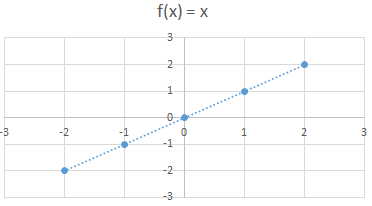
\includegraphics[width=0.7\linewidth]{1_elem_rekenvaardigheden_A/inputs/absValue}
%		\caption{Absolute waarde - voorbeeld 1.}
%		\label{fig:absvalue}
%	\end{figure}	
\end{voorbeeld}

\begin{voorbeeld}
	Zie Figuur \ref{fig:absvalue2}
	\figuurmetlabel[\label{fig:absvalue2}]{width=7cm}{1_elem_rekenvaardigheden_A/inputs/absValue2}{Absolute waarde - voorbeeld 2.}
%	\begin{figure}
%	\centering
%	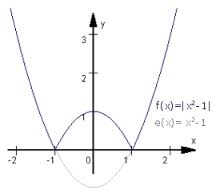
\includegraphics[width=0.7\linewidth]{1_elem_rekenvaardigheden_A/inputs/absValue2}
%	\caption{Absolute waarde - voorbeeld 2.}
%	\label{fig:absvalue2}
%	\end{figure}	
\end{voorbeeld}

\subsection{Sommatie}

Een sommatie is het sommeren of optellen van een groep getallen. 
In de wiskunde wordt een sommatie aangegeven met de griekse hoofdletter sigma: $\sum$ 

\begin{notatie}
Voor getallen $x_m,x_{m+1},\ldots,x_n$ voeren we volgende notatie in
\begin{equation*}
\sum_{i=m}^{n}x_i = x_m + x_{m+1} + x_{m+2} + \ldots + x_{n-2} + x_{n-1} + x_{n}
\end{equation*}	
\end{notatie}

\begin{voorbeeld}
	\begin{equation*}
	\sum_{i=1}^{100}i = 1+2+3+\ldots+100
	\end{equation*}
	De $i$ duidt de index aan. Deze begint te tellen vanaf de ondergrens (in dit voorbeeld 1) tot en met de bovengrens (hier dus 100). Het verhogen gebeurt steeds in stapjes van 1.
	
\end{voorbeeld}

\begin{voorbeeld}
	Soms begint men liever vanaf nul te tellen. In dat geval kan je zelf gemakkelijk de formule en grenzen aanpassen:
	
		\begin{equation*}
	\sum_{i=1}^{100}i = 1+2+3+\ldots+100
	\end{equation*}
	
wordt dan

	\begin{equation*}
\sum_{i=0}^{99} (i+1) = 1+2+3+\ldots+100
\end{equation*}

\end{voorbeeld}

Hieronder worden nog een aantal andere voorbeelden gegeven. Je kan zelf ook eindeloos voorbeelden blijven bedenken.

\begin{voorbeeld}
	\begin{equation*}
	\sum_{i=1}^{10} 4^i = 4^1+4^2+4^3+\ldots+4^{10}
	\end{equation*}
	\begin{equation*}
	\sum_{i=0}^{10} x^{2i} = x^0+x^2+x^4+\ldots+x^{20}
	\end{equation*}
\end{voorbeeld}

In de statistiek wordt vaak gebruik gemaakt van het gemiddelde. Om het gemiddelde $\overline{x}$ van $n$ getallen te berekenen, maak je gebruik van volgende formule:

\begin{equation*}
\overline{x} = \frac{(x_1+x_2+\ldots+x_n)}{n}=\frac{1}{n}(x_1+x_2+\ldots+x_n)
\end{equation*}

Door gebruik te maken van het sommatieteken kan je dit korter noteren:

\begin{equation*}
\overline{x}=\sum_{i=1}^{n}\frac{x_i}{n} = \frac{1}{n} \sum_{i=1}^{n} x_n
\end{equation*}

Hieruit volgt dat je een gemeenschappelijke constante (in dit geval $\frac{1}{n}$) gewoon buiten de eigenlijke sommatie kan plaatsen.



\subsection{Sommatie - voorbeeld}
\begin{minipage}{.25\linewidth}
	\raggedright
	
\includegraphics[width=4cm]{1_elem_rekenvaardigheden_A/inputs/QR_Code_SOMMATIE_module_1}
\end{minipage}
\begin{minipage}{.7\linewidth}
	Zie filmpje MOOC.
\end{minipage}

\subsection{Faculteit}
In dit onderdeel wordt dieper ingegaan op rekenen met faculteiten en indien mogelijk het vereenvoudigen van faculteiten.

\begin{definitie}
	De faculteit van een natuurlijk getal $n$, genoteerd als $n!$ (lees “$n$ faculteit”), is gedefinieerd als het product van de getallen 1 tot en met $n$:
	\begin{equation*}
	n!=n.(n-1)\cdot(n-2)\cdot(n-3)\cdot\ldots\cdot 3\cdot 2\cdot 1
	\end{equation*}
\end{definitie}

De faculteit van $n$ kan je ook met een recursief voorschrift schrijven: $n!=n(n-1)!$

We noemen een voorschrift recursief als er een verband bestaat met vorige resultaten: aangezien $5!=120$ is, geldt
\begin{equation*}
6!=6\cdot 5!=6\cdot 120=720
\end{equation*}
Maar dit recursief gedrag vraagt dat $1!=1\cdot 0!$ Daarom is per definitie gesteld dat:

\begin{definitie}
	0!=1
\end{definitie}

De faculteitsfunctie groeit snel, zelfs sneller dan een exponenti\"ele functie.  $20!$ is een getal van reeds 19 cijfers, terwijl $1000!$ zo'n 2568 cijfers telt.

Het getal $n$ behoort tot de natuurlijke getallen en is dus altijd een positief geheel getal.
Met dit in het achterhoofd kijken we even naar het volgende voorbeeld:

\begin{equation*}
-(3!)=-(3\cdot 2\cdot 1)=-6
\end{equation*}

$(-3)!$ heeft geen betekenis want tussen de haakjes staat een negatief geheel getal en dit behoort niet tot de verzameling van natuurlijke getallen.

\begin{voorbeeld}
	\begin{equation*}
	\frac{6!}{3!}=\frac{6\cdot 5\cdot 4\cdot 3\cdot 2\cdot 1}{3\cdot 2\cdot 1} = 6\cdot 5\cdot 4 = 120
	\end{equation*}
	Let op! Je ziet dus dat je $\frac{6!}{3!}$ niet kan behandelen als een gewone breuk en dat bijgevolg $2!$ een foutief antwoord zou zijn.
\end{voorbeeld}

\begin{voorbeeld}
Een meer algemeen voorbeeld is:
\begin{equation*}
\frac{(n+1)!}{(n-1)!}=\frac{(n+1) \cdot n\cdot (n-1)!}{(n-1)!}=n(n+1)
\end{equation*}
\end{voorbeeld}

Als de faculteitsfunctie $n!$ zo snel toeneemt, dan zal $\frac{1}{n!}$ overeenkomstig ook snel afnemen.

Wiskundig kan je je dan afvragen wat er gebeurt als $n$ oneindig groot wordt. Dit soort vragen zal leiden tot het limietbegrip en notaties als:
\begin{equation*}
\lim\limits_{n \to +\infty} \frac{1}{n!}
\end{equation*}

En wat zou er gebeuren mocht je al deze getallen bij elkaar optellen? Dus waaraan zou volgende som gelijk zijn:

\begin{equation*}
\sum_{=0}^{\infty} \frac{1}{n!} = 1+1+\frac{1}{2!}+\frac{1}{3!}+\ldots=?
\end{equation*}

Dit blijkt het getal $e=2,718\ldots$ te zijn.

Andere toepassingen van de faculteitsfunctie vinden we terug in het vak statistiek en meer bepaald de combinatieleer. Een vaak voorkomende vraag is hier \textquotedblleft op hoeveel verschillende manieren kan je $k$ voorwerpen ordenen?\textquotedblright \  Een voorbeeld: je hebt 2 foto's op je bureau staan. Op hoeveel manieren kan je deze plaatsen? Het antwoord is op $2!=2$ manieren. Met 3 foto's heb je $3!=6$ manieren, en met 10 foto's zijn er al $10!=3628800$ mogelijkheden.

\subsection{Vectoren vs scalairen}
\subsubsection{Wat is een scalair?}
In wetenschap en techniek gebruikt men vaak grootheden die volledig bepaald zijn door \'e\'en re\"eel getal. Degelijke grootheden noemt men scalaire grootheden. Een scalaire grootheid heeft enkel een grootte.

\begin{voorbeeld}
$m=20kg$ (massa), $V=10l$ (volume), $T=35$\textdegree$C$ (temperatuur)
\end{voorbeeld}

\subsubsection{Wat is een vector?}

\begin{definitie}
	We defini\"eren een vector als een grootheid bepaald door een richting, een zin en een grootte.
\end{definitie}

\begin{voorbeeld}
	$\vec{v}=20 m/s$ (snelheid), $\vec{F}=5N$ (kracht), $\vec{E}=20 N/C$ (elektrisch veld)
\end{voorbeeld}

\begin{opmerking}
	\ \\
\begin{itemize}
	\item Een vector is een pijl die twee punten $A$ en $B$ verbindt. Vectoren worden genoteerd door een letter met een pijltje erboven bv. $\vec{v}$. We kunnen ook kiezen om het begin- en eindpunt op te nemen in de notatie. We noteren $\vec{v}=\vec{AB}$.
	\item Een vector $\vec{v}$ wordt volledig bepaald door de grootte, richting en de zin. Twee vectoren zijn dus identiek wanneer hun grootte, hun richting en hun zin dezelfde zijn.
	\item In het algemeen heeft een vector geen positie, men spreekt dan van een \textbf{vrije vector}. Het aangrijpingspunt is niet bepaald. De vrije vectoren behoren tot de verzameling $V$.
	\item De verzameling punten van het vlak noteren we door $\pi$. Kiest men in het vlak $\pi$ een bevoorrecht punt $O$ dan ontstaat het vlak $\pi_O$. Men legt dus de oorsprong  vast in het vlak, en laat alle vector beginnen in de oorsprong. Het punt $P$ in het vlak kunnen we bekijken als het eindpunt van deze vector, namelijk de vector $\vec{OP}=\vec{P}$. Een dergelijke vector noemen we in de wiskunde een \textbf{gebonden} vector, een \textbf{vaste} vector, een \textbf{puntvector} of een \textbf{plaatsvector}. De puntvectoren behoren tot de verzameling $\pi_O$.
	\item De vector $\vec{AA}$ wordt aangeduid met $\vec{O}$ en heeft als lengte 0. Zo een vector noemen we een \textbf{nulvector}. De samenstelling van een vector met een nulvector levert de oorspronkelijke vector op: $\vec{AB}+\vec{O}$. De nulvector is het neutraal element voor de optelling.
	\item Beschouwen we een vector $\vec{AB}$. De vector $\vec{BA}=-\vec{AB}$ met dezelfde richting en grootte, maar met tegengestelde zin wordt de tegengestelde vector genoemd. De samenstelling van een vector met zijn tegengestelde vector levert de nulvector op: $\vec{AB}+\vec{BA}=\vec{O}$.
	\item Een eenheidsvector is een vector met lengte \'e\'en. Eenheidsvectoren worden vooral gebruikt om een richting aan te geven. Een vector met willekeurige niet-nulle norm kan worden gedeeld door zijn norm om zo een eenheidsvector te cre\"eren. Dit proces staat bekend als het normaliseren van een vector. Een eenheidsvector wordt vaak aangeduid met een hoedje, zoals in $\hat{a}$  of ook door $\vec{e_1}$ (of $\vec{1_x}$ als het over de eenheidsvector volgens de $x$-as gaat).
	\begin{equation*}
	\hat{a} = \frac{\vec{a}}{||\vec{a}||}
	\end{equation*}
	\item De lengte of de norm van een vector $\vec{AB}$ of $\vec{v}$ noteert men door $||\vec{AB}||$ of $||\vec{v}||$.
\end{itemize}	
\end{opmerking}

\subsubsection{Bewerkingen met vectoren}

\emph{De optelling}

\begin{definitie}
De som van twee vectoren is opnieuw een vector: $\vec{v_1}+\vec{v_2}=\vec{v}$

Het verschil van twee vectoren is opnieuw een vector. $\vec{v_1}-\vec{v_2}=\vec{v_1}+(-\vec{v_2})=\vec{v}$
\end{definitie}

\begin{opmerking}
	Let op! $||\vec{v_1}||+||\vec{v_2}|| \ne ||\vec{v}||$
\end{opmerking}

Het samenstellen van twee vectoren gebeurt volgens de \textbf{parallellogramregel}, zie Figuur \ref{fig:som_par}. Wanneer we twee vectoren $\vec{v_1}$ en $\vec{v_2}$ (met een verschillende richting) willen optellen, dan construeren we een parallellogram. We plaatsen $\vec{v_1}$ en $\vec{v_2}$ zodat hun aangrijpingspunt samenvalt. De som $\vec{v_1}+\vec{v_2}$ wordt dan gegeven door de vector met het aangrijpingspunt en eindpunt het overstaand hoekpunt van de parallellogram.

\figuurmetlabel[\label{fig:som_par}]{width=7cm}{1_elem_rekenvaardigheden_A/inputs/parRegelSom}{Parallellogramregel voor het bepalen van de som van 2 vectoren.}

Deze parallellogram constructie kan ook gebruikt worden voor het omgekeerde proces, namelijk het \textbf{ontbinden van een vector in 2 (of meerdere) componenten (dit zijn scalairen)}, elk volgens een bepaalde richting. Vaak wordt dan een gegeven vector ontbonden in een component volgens de $x$-as en een component volgens de $y$-as.

\figuurmetlabel[\label{fig:kopstaartsom_par}]{width=7cm}{1_elem_rekenvaardigheden_A/inputs/kopstaart}{Kopstaartregel voor het bepalen van de som van 2 vectoren.}

Een andere manier om twee vectoren op te tellen, is deze kop aan staart te leggen, zie Figuur \ref{fig:kopstaart}. We plaatsen de vector $\vec{v_2}$ zodat zijn beginpunt samenvalt met het eindpunt van de vector $\vec{v_1}$. De som  wordt dan gegeven door de vector wijzend van het beginpunt van $\vec{v_1}$ naar het eindpunt van $\vec{v_2}$. Deze regel noemen we de \textbf{driehoeksregel} of de \textbf{kopstaartregel}.

\emph{De vermenigvuldiging van een vector met een scalair}

\begin{definitie}
	Wanneer men een vector $\vec{v}$ vermenigvuldigt met een scalair $k$, krijgt men de nieuwe vector $k\vec{v}$. 
	
	De grootte van deze nieuwe vector is $k||\vec{v}||$.
	
	De richting verandert niet, terwijl de zin omdraait als $k<0$ (lees “als $k$ negatief is”).
\end{definitie}

\begin{opmerking}
	Let op! een scalaire vermenigvuldiging mag je niet verwarren met het scalair product (zie verder)
\end{opmerking}

\emph{De vermenigvuldiging van twee vectoren}

\begin{definitie}
	\ \\
\begin{enumerate}
	\item het scalair product of inwendig product:
	\begin{equation*}
	\vec{v_1} \cdot \vec{v_2} = ||\vec{v_1}|| \cdot  ||\vec{v_2}|| \cdot \cos \theta = \text{getal}
	\end{equation*}
	Hierbij is $\theta$ de hoek tussen de 2 vectoren. Het scalair product is dus maximaal als beide vectoren in dezelfde richting wijzen (met andere woorden parallel zijn). En anderzijds is het scalair product nul als beide vectoren loodrecht op elkaar staan.

	\item het vectorieel product, kruisproduct of uitwendig product:
	\begin{equation*}
	\vec{v_1} \times \vec{v_2} = \begin{vmatrix}
	\vec{e_1} & \vec{e_2} & \vec{e_3} \\
	a_1 & a_2 & a_3 \\
	b_1 & b_2 & b_3 
	\end{vmatrix} = \text{vector}
	\end{equation*} 
\end{enumerate}
\end{definitie}
De eigenschappen van de nieuwe vector zijn:

\begin{enumerate}
	\item Over de richting van $\vec{a} \times \vec{b}$: het staat loodrecht op $\vec{a}$ en $\vec{b}$.
	\item Over de zin van $\vec{a} \times \vec{b}$: $\vec{a}$, $\vec{b}$  en $\vec{a} \times \vec{b}$ vormen een rechtshandig assenstelsel.
	\item De norm van $\vec{a} \times \vec{b}$ is $||\vec{a} \times \vec{b}||=||\vec{a}||\cdot||\vec{b}||\cdot \sin \theta$, waarin $\theta$ de hoek is tussen $\vec{a}$ en $\vec{b}$.
\end{enumerate}
Het vectorieel product is dus maximaal als beide vectoren loodrecht op elkaar staan. En anderzijds is het vectorieel product nul als beide vectoren evenwijdig zijn (en dus dezelfde richting hebben).

\subsection{Ontbinden van een vector - voorbeeld}
\begin{minipage}{.25\linewidth}
	\raggedright
	
\includegraphics[width=4cm]{1_elem_rekenvaardigheden_A/inputs/QR_Code_ONTBINDEN_module_1}
\end{minipage}
\begin{minipage}{.7\linewidth}
	Zie filmpje MOOC.
\end{minipage}

\subsection{Test - wiskundige notaties}
TODO